\documentclass[a4paper]{article}
\usepackage[a4paper,margin=0mm]{geometry}
\usepackage{fontspec}
\usepackage{unicode-math}
\usepackage{tikz}
\usetikzlibrary{calc}
\usepackage[table]{xcolor}
\usepackage[absolute]{textpos}
\usepackage{enumitem}
\usepackage{array}
\usepackage{multirow}

\setmainfont{Libertinus Serif}
\setsansfont{Libertinus Sans}
\setmathfont{Libertinus Math}

\definecolor{accent}{HTML}{0F6A52}
\definecolor{badge}{HTML}{A9CFC2}
\definecolor{ink}{HTML}{2A2E30}

\setlength{\TPHorizModule}{1mm}
\setlength{\TPVertModule}{1mm}
\setlength{\parindent}{0pt}
\pagestyle{empty}
\binoppenalty=10000 \relpenalty=10000

\newcommand{\LCOL}{16mm}
\newcommand{\RCOL}{111mm}
\newcommand{\COLW}{83mm}

\newcommand{\topicheader}[2]{%
\begin{textblock*}{194mm}(16mm,10mm)
\begin{tikzpicture}
\node[fill=accent,text=white,font=\sffamily\bfseries\fontsize{13}{13}\selectfont,
      minimum width=9mm,minimum height=9mm,inner sep=0pt] at (4.5mm,-4.5mm) {#1};
\node[font=\sffamily\bfseries\fontsize{15}{16}\selectfont,text=ink,anchor=west] at (12mm,-4.5mm) {#2};
\end{tikzpicture}
\end{textblock*}
\begin{textblock*}{194mm}(16mm,22.5mm)

\begin{tikzpicture}
\fill[accent] (0,0) rectangle (194mm,0.5mm);
\end{tikzpicture}
\end{textblock*}
}

\newcommand{\pagefooter}[1]{%
\begin{textblock*}{194mm}(8mm,286.41mm)
  
\begin{tikzpicture}
    \fill[accent] (0,0) rectangle (194mm,0.6mm);
  \end{tikzpicture}
\end{textblock*}
\begin{textblock*}{63.59mm}(8mm,288.27mm)
  {\sffamily\bfseries\color{accent}\fontsize{13}{16}\selectfont SAT 1200+}
\end{textblock*}
\begin{textblock*}{10mm}(188mm,288.27mm)
  \centering{\sffamily\color{accent}\fontsize{14}{16}\selectfont #1}
\end{textblock*}
}

\newcommand{\colrule}[2]{%
\begin{textblock*}{1mm}(105mm,#1mm)
\begin{tikzpicture}
\draw[black!65,line width=0.5pt] (0,0) -- (0,#2mm);
\end{tikzpicture}
\end{textblock*}
}

% Page kicker: left = module line, right = question range
\newcommand{\pagekicker}[2]{%
\begin{textblock*}{194mm}(16mm,25.2mm)
{\sffamily\bfseries\fontsize{10.5}{12}\selectfont\color{accent}#1}\hfill{\sffamily\fontsize{10}{12}\selectfont\color{black!70}#2}
\end{textblock*}
}

\setlength{\fboxsep}{1.4pt}
\setlength{\fboxrule}{0.5pt}
\newcommand{\pnum}[1]{\fcolorbox{ink}{white}{\sffamily\bfseries\fontsize{8}{8}\selectfont #1}~}

% centered display line inside a stem
\newcommand{\dsp}[1]{\par\vspace{1.4mm}\centerline{#1}\vspace{1.8mm}}

% student-produced response box
\newcommand{\gridbox}{%
\par\vspace{3mm}\noindent

\begin{tikzpicture}
\node[anchor=south west,font=\sffamily\bfseries\fontsize{7.5}{9}\selectfont,text=accent,inner sep=0pt] at (0,0.3mm) {STUDENT-PRODUCED RESPONSE};
\draw[ink,line width=0.7pt] (0,-9.5mm) rectangle (40mm,-0.8mm);
\node[anchor=west,font=\sffamily\fontsize{7.5}{9}\selectfont,text=black!55,inner sep=0pt] at (43mm,-5.2mm) {Write your answer in the box.};
\end{tikzpicture}\par}

\arrayrulecolor{accent}
\setlength{\arrayrulewidth}{0.7pt}
\renewcommand{\arraystretch}{1.35}

\newcommand{\figwrap}[1]{\par\vspace{2.5mm}\centerline{{\arrayrulecolor{ink}\setlength{\arrayrulewidth}{0.5pt}\renewcommand{\arraystretch}{1.3}#1}}\vspace{0.5mm}}

\begin{document}

% ================= PAGE 1: Mock Test 9 -- instructions + geometry reference sheet =================
\topicheader{9}{Mock Test 9}
\pagefooter{214}
\mbox{}%

\newcommand{\cardhead}[1]{{\sffamily\bfseries\color{accent}\fontsize{11.5}{14}\selectfont #1}\par\vspace{0.6mm}%
{\color{accent}\rule{\linewidth}{0.5pt}}\par\vspace{1.6mm}}
\newcommand{\bul}{\item[\textcolor{accent}{\rule[0.2mm]{1.5mm}{1.5mm}}]}

\begin{textblock*}{194mm}(16mm,28mm)
{\sffamily\bfseries\color{accent}\fontsize{26}{28}\selectfont Mock Test 9\par}
\vspace{1mm}
{\sffamily\color{ink}\fontsize{11}{14}\selectfont Full-length digital SAT Math practice \;\textperiodcentered\; 2 modules $\times$ 22 questions $\times$ 35 minutes\par}
\end{textblock*}

\begin{textblock*}{\COLW}(\LCOL,53mm)
{\fontsize{9.4}{12.2}\selectfont
\cardhead{How this test works}
\renewcommand{\arraystretch}{1.3}\setlength{\tabcolsep}{4pt}
\noindent\begin{tabular}{|>{\raggedright\arraybackslash}p{20mm}|>{\centering\arraybackslash}p{15mm}|>{\centering\arraybackslash}p{13mm}|>{\centering\arraybackslash}p{19mm}|}
\hline
\rowcolor{badge!55}\textbf{Module} & \textbf{Questions} & \textbf{Time} & \textbf{Calculator}\\\hline
Module 1 & 22 & 35 min & allowed\\\hline
Module 2 & 22 & 35 min & allowed\\\hline
\end{tabular}\par\vspace{2.2mm}
\begin{itemize}[leftmargin=5mm,itemsep=1.2mm,topsep=0mm,parsep=0mm]
\bul Time each module separately: 35 minutes, not a minute more. Rest for 5--10 minutes between the two modules.
\bul Use a calculator (the built-in Desmos graphing calculator or any approved calculator) on both modules.
\bul Module 1 is a standard mix of easy, medium and hard questions. Module 2 is the \emph{harder route} you reach by doing well on Module 1.
\bul Answer every question. There is no penalty for a wrong answer.
\bul Unless a problem says otherwise, all numbers are real, a function's domain is every real number for which it is defined, and figures are not necessarily drawn to scale.
\bul Do not look at any answers while you work. When you finish both modules, score yourself with the \textbf{Answer Sheets} section at the end of this book.
\end{itemize}
}
\end{textblock*}

\begin{textblock*}{\COLW}(\RCOL,53mm)
{\fontsize{9.4}{12.2}\selectfont
\cardhead{Student-produced responses (grid-ins)}
Some questions have no answer choices. Work out the answer and write it in the answer box (on the real test you type it in).
\begin{itemize}[leftmargin=5mm,itemsep=1.2mm,topsep=1.6mm,parsep=0mm]
\bul You may give an integer, a decimal, or a fraction. For one answer, $9/2$ and $4.5$ are both correct.
\bul Never enter a mixed number: write $7/2$ or $3.5$, not $3\,1/2$ (it would be read as $31/2$).
\bul Do not enter symbols or units such as \$, \%, or $\pi$. Enter the number only.
\bul An answer may use at most 5 characters (6 if it is negative), counting the slash and the decimal point.
\bul If an answer is a repeating decimal, enter it as a fraction such as $2/3$, or fill all the digits that fit: $0.6666$ or $0.6667$.
\bul If you find more than one correct answer, enter only one of them.
\end{itemize}
\vspace{1.2mm}
\noindent\fcolorbox{accent}{badge!25}{\parbox{\dimexpr\linewidth-2\fboxsep-2\fboxrule}{\centering\sffamily\fontsize{8.5}{11}\selectfont
\textbf{Example.} Answer $4\tfrac12$ \;$\rightarrow$\; enter \textbf{9/2} or \textbf{4.5}\par}}
\par\vspace{3mm}
\noindent{\sffamily\bfseries\color{accent}Pacing.}\ Q1--15: about 18 min. Q16--22: about 17 min. Keep the last 2--3 min for flagged questions and every blank grid-in (a blank is a guaranteed zero).
}
\end{textblock*}

% ---- Geometry reference sheet (full width card) ----
\begin{textblock*}{178mm}(16mm,156mm)
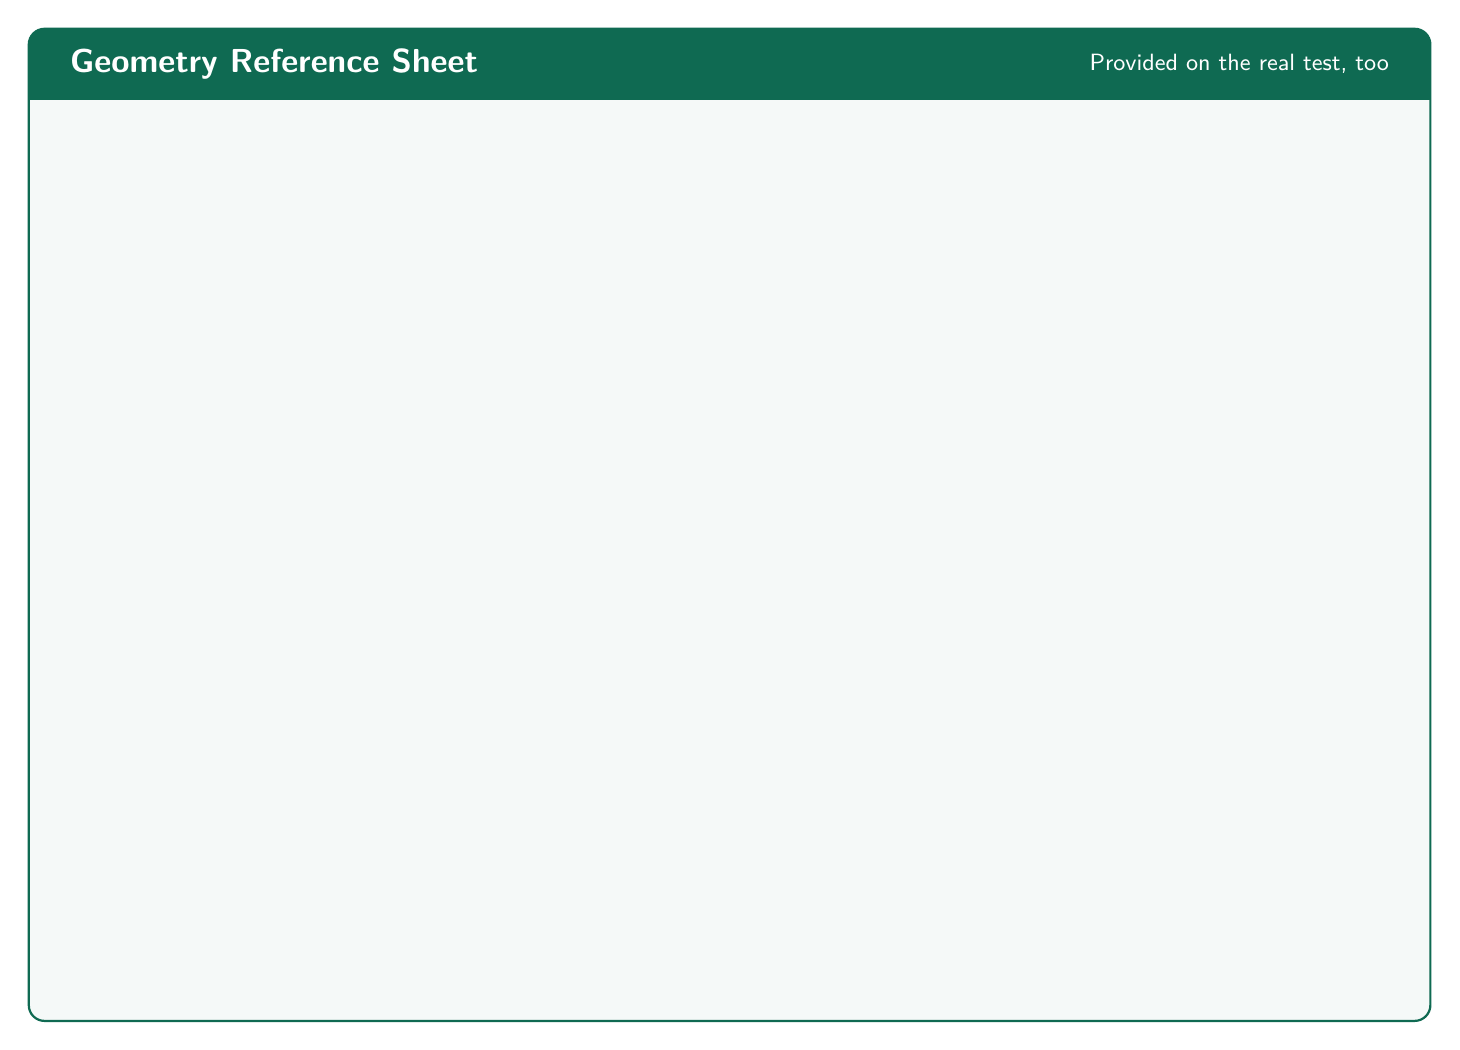
\begin{tikzpicture}
\draw[accent,line width=0.8pt,rounded corners=2mm,fill=badge!12] (0,0) rectangle (178mm,-126mm);
\fill[accent,rounded corners=2mm] (0,0) rectangle (178mm,-9mm);
\fill[accent] (0,-5mm) rectangle (178mm,-9mm);
\node[anchor=west,text=white,font=\sffamily\bfseries\fontsize{12}{14}\selectfont] at (4mm,-4.5mm) {Geometry Reference Sheet};
\node[anchor=east,text=white,font=\sffamily\fontsize{8.5}{10}\selectfont] at (174mm,-4.5mm) {Provided on the real test, too};
\end{tikzpicture}
\end{textblock*}

\newcommand{\refcell}[3]{\begin{textblock*}{42mm}(#1mm,#2mm)\begin{minipage}[t][36mm][t]{42mm}\centering #3\end{minipage}\end{textblock*}}
\newcommand{\refin}[2]{\parbox[b][26mm][b]{42mm}{\centering #1}\par\vspace{1.6mm}{\fontsize{9.6}{11.5}\selectfont #2}}
\tikzset{rf/.style={ink,line width=0.65pt},lb/.style={font=\fontsize{8.5}{9.5}\selectfont,inner sep=1.2pt}}

% ---------- row 1
\refcell{18}{167}{\refin{\begin{tikzpicture}[scale=1.25]
\draw[rf] (0,0) circle (9mm); \draw[rf] (0,0)--(9mm,0); \fill[ink] (0,0) circle (0.7pt);
\node[lb,above] at (4.5mm,0) {$r$};
\end{tikzpicture}}{Circle\\$A=\pi r^{2}$,\; $C=2\pi r$}}
\refcell{62}{167}{\refin{\begin{tikzpicture}[scale=1.25]
\draw[rf] (0,0) rectangle (22mm,12mm);
\node[lb,below] at (11mm,0) {$\ell$}; \node[lb,right] at (22mm,6mm) {$w$};
\end{tikzpicture}}{Rectangle\\$A=\ell w$}}
\refcell{106}{167}{\refin{\begin{tikzpicture}[scale=1.25]
\draw[rf] (0,0)--(22mm,0)--(7mm,13mm)--cycle;
\draw[rf,dashed] (7mm,0)--(7mm,13mm);
\draw[rf] (7mm,0)++(0,1.8mm)--++(1.8mm,0)--++(0,-1.8mm);
\node[lb,below] at (11mm,0) {$b$}; \node[lb,left] at (7mm,6.5mm) {$h$};
\end{tikzpicture}}{Triangle\\$A=\tfrac12 bh$}}
\refcell{150}{167}{\refin{\begin{tikzpicture}[scale=1.25]
\draw[rf] (0,0)--(18mm,0)--(0,12mm)--cycle;
\draw[rf] (0,1.8mm)--(1.8mm,1.8mm)--(1.8mm,0);
\node[lb,below] at (9mm,0) {$a$}; \node[lb,left] at (0,6mm) {$b$}; \node[lb,above right] at (9mm,6mm) {$c$};
\end{tikzpicture}}{Right triangle\\$c^{2}=a^{2}+b^{2}$}}

% ---------- row 2
\refcell{18}{204}{\refin{\begin{tikzpicture}[scale=1.25]
\draw[rf] (0,0)--(19.053mm,0)--(0,11mm)--cycle;
\draw[rf] (0,1.8mm)--(1.8mm,1.8mm)--(1.8mm,0);
\node[lb,below] at (9.5mm,0) {$x\sqrt3$}; \node[lb,left] at (0,5.5mm) {$x$}; \node[lb,above right] at (9.5mm,5.5mm) {$2x$};
\node[lb] at (14.6mm,1.9mm) {\fontsize{6.5}{7}\selectfont$30^\circ$}; \node[lb] at (3.2mm,8.2mm) {\fontsize{6.5}{7}\selectfont$60^\circ$};
\end{tikzpicture}}{$30^\circ$--$60^\circ$--$90^\circ$ triangle}}
\refcell{62}{204}{\refin{\begin{tikzpicture}[scale=1.25]
\draw[rf] (0,0)--(10mm,0)--(0,10mm)--cycle;
\draw[rf] (0,1.8mm)--(1.8mm,1.8mm)--(1.8mm,0);
\node[lb,below] at (5mm,0) {$s$}; \node[lb,left] at (0,5mm) {$s$}; \node[lb,above right] at (5mm,5mm) {$s\sqrt2$};
\end{tikzpicture}}{$45^\circ$--$45^\circ$--$90^\circ$ triangle}}
\refcell{106}{204}{\refin{\begin{tikzpicture}[scale=1.2]
\draw[rf] (0,0) rectangle (16mm,9mm);
\draw[rf] (16mm,9mm)--(22mm,13mm)--(6mm,13mm)--(0,9mm);
\draw[rf] (16mm,0)--(22mm,4mm)--(22mm,13mm);
\draw[rf,dashed] (6mm,13mm)--(6mm,4mm)--(22mm,4mm); \draw[rf,dashed] (0,0)--(6mm,4mm);
\node[lb,below] at (8mm,0) {$\ell$}; \node[lb,right] at (22mm,8.5mm) {$h$}; \node[lb,below right] at (19mm,2mm) {$w$};
\end{tikzpicture}}{Rectangular solid\\$V=\ell wh$}}
\refcell{150}{204}{\refin{\begin{tikzpicture}[scale=1.2]
\draw[rf] (0,2.2mm) ellipse (7mm and 2.2mm);
\draw[rf] (-7mm,2.2mm)--(-7mm,14mm); \draw[rf] (7mm,2.2mm)--(7mm,14mm);
\draw[rf] (0,14mm) ellipse (7mm and 2.2mm);
\draw[rf,dashed] (0,14mm)--(7mm,14mm); \fill[ink] (0,14mm) circle (0.6pt);
\node[lb,above] at (3.5mm,14mm) {$r$}; \node[lb,right] at (7mm,8mm) {$h$};
\end{tikzpicture}}{Right circular cylinder\\$V=\pi r^{2}h$}}

% ---------- row 3
\refcell{18}{241}{\refin{\begin{tikzpicture}[scale=1.15]
\draw[rf] (0,0) circle (10mm);
\draw[rf] (-10mm,0) arc (180:360:10mm and 2.8mm); \draw[rf,dashed] (-10mm,0) arc (180:0:10mm and 2.8mm);
\draw[rf] (0,0)--(10mm,0); \fill[ink] (0,0) circle (0.7pt); \node[lb,above] at (5mm,0) {$r$};
\end{tikzpicture}}{Sphere\\$V=\tfrac43\pi r^{3}$}}
\refcell{62}{241}{\refin{\begin{tikzpicture}[scale=1.2]
\draw[rf] (0,2.2mm) ellipse (7mm and 2.2mm);
\draw[rf] (-7mm,2.2mm)--(0,16mm)--(7mm,2.2mm);
\draw[rf,dashed] (0,16mm)--(0,2.2mm); \draw[rf,dashed] (0,2.2mm)--(7mm,2.2mm);
\fill[ink] (0,2.2mm) circle (0.6pt);
\node[lb,left] at (0,9.5mm) {$h$}; \node[lb,above] at (3.5mm,2.2mm) {$r$};
\end{tikzpicture}}{Right circular cone\\$V=\tfrac13\pi r^{2}h$}}
\refcell{106}{241}{\refin{\begin{tikzpicture}[scale=1.2]
\draw[rf] (0,0)--(16mm,0)--(22mm,4mm); \draw[rf] (0,0)--(10mm,15mm)--(16mm,0); \draw[rf] (10mm,15mm)--(22mm,4mm);
\draw[rf,dashed] (0,0)--(6mm,4mm)--(22mm,4mm); \draw[rf,dashed] (6mm,4mm)--(10mm,15mm);
\node[lb,below] at (8mm,0) {$\ell$}; \node[lb,below right] at (19mm,2mm) {$w$}; \node[lb,left] at (10mm,9.5mm) {$h$};
\end{tikzpicture}}{Rectangular pyramid\\$V=\tfrac13\ell wh$}}
\begin{textblock*}{40mm}(151mm,247mm)
{\fontsize{9.2}{12}\selectfont\raggedright
\textcolor{accent}{\rule[0.3mm]{1.6mm}{1.6mm}}\; A circle has 360 degrees of arc.\par\vspace{1.2mm}
\textcolor{accent}{\rule[0.3mm]{1.6mm}{1.6mm}}\; The angles of a triangle add up to 180 degrees.\par\vspace{1.2mm}
\textcolor{accent}{\rule[0.3mm]{1.6mm}{1.6mm}}\; $r$ radius, $\ell$ length, $w$ width, $b$ base, $h$ height.\par}
\end{textblock*}

\clearpage

% ===== Module 1, page 1 =====
\topicheader{9}{Mock Test 9}
\pagefooter{215}
\colrule{34}{236}
\mbox{}%
\pagekicker{Mock 9 \textperiodcentered{} Module 1 \textperiodcentered{} 22 questions \textperiodcentered{} 35 minutes}{Questions 1--8}
\begin{textblock*}{\COLW}(\LCOL,34mm)
{\fontsize{10.4}{13.4}\selectfont
\parbox[t][233mm][t]{\COLW}{%
\noindent\pnum{1} An event planner charges a flat fee of \$180 plus \$12 for each guest. A client paid a total of \$540. How many guests were there?\par\vspace{2.2mm}
\hspace*{7mm}(A)\ $45$\\[1.8mm]
\hspace*{7mm}(B)\ $30$\\[1.8mm]
\hspace*{7mm}(C)\ $60$\\[1.8mm]
\hspace*{7mm}(D)\ $360$
\vfill

\noindent\pnum{2} Which of the following is equivalent to $(x-3)(x+8)$?\par\vspace{2.2mm}
\hspace*{7mm}(A)\ $x^{2}+11x-24$\\[1.8mm]
\hspace*{7mm}(B)\ $x^{2}-5x-24$\\[1.8mm]
\hspace*{7mm}(C)\ $x^{2}-24$\\[1.8mm]
\hspace*{7mm}(D)\ $x^{2}+5x-24$
\vfill

\noindent\pnum{3} A clothing store has 480 jackets in stock at the start of a clearance sale. By the end of the sale, 35\% of the jackets have been sold. How many jackets are left in stock?\gridbox
\vfill

\noindent\pnum{4} A rectangular loading dock has a perimeter of 62 meters and a width of 11 meters. What is the area of the dock, in square meters?\par\vspace{2.2mm}
\hspace*{7mm}(A)\ $220$\\[1.8mm]
\hspace*{7mm}(B)\ $341$\\[1.8mm]
\hspace*{7mm}(C)\ $440$\\[1.8mm]
\hspace*{7mm}(D)\ $682$
\vfill}}
\end{textblock*}
\begin{textblock*}{\COLW}(\RCOL,34mm)
{\fontsize{10.4}{13.4}\selectfont
\parbox[t][233mm][t]{\COLW}{%
\noindent\pnum{5} The temperature in degrees Fahrenheit, $F$, is related to the temperature in degrees Celsius, $C$, by the equation $F=1.8C+32$. A greenhouse is kept at $86^{\circ}$F. What is this temperature in degrees Celsius?\par\vspace{2.2mm}
\hspace*{7mm}(A)\ $54$\\[1.8mm]
\hspace*{7mm}(B)\ $65.6$\\[1.8mm]
\hspace*{7mm}(C)\ $30$\\[1.8mm]
\hspace*{7mm}(D)\ $79.8$
\vfill

\noindent\pnum{6} If $2^{x}=32$, what is the value of $2^{x-2}$?\par\vspace{2.2mm}
\hspace*{7mm}(A)\ $8$\\[1.8mm]
\hspace*{7mm}(B)\ $30$\\[1.8mm]
\hspace*{7mm}(C)\ $16$\\[1.8mm]
\hspace*{7mm}(D)\ $3$
\vfill

\noindent\pnum{7} A delivery van leaves the depot carrying 240 packages. At each stop it drops off 8 packages and picks up none. After how many stops will exactly 72 packages remain on the van?\gridbox
\vfill

\noindent\pnum{8} For $x>0$, which of the following is equivalent to $\sqrt{x}\cdot x^{3/2}$?\par\vspace{2.2mm}
\hspace*{7mm}(A)\ $x^{3/4}$\\[1.8mm]
\hspace*{7mm}(B)\ $x^{2}$\\[1.8mm]
\hspace*{7mm}(C)\ $x^{5/2}$\\[1.8mm]
\hspace*{7mm}(D)\ $x$
\vfill}}
\end{textblock*}
\clearpage

% ===== Module 1, page 2 =====
\topicheader{9}{Mock Test 9}
\pagefooter{216}
\colrule{34}{236}
\mbox{}%
\pagekicker{Mock 9 \textperiodcentered{} Module 1 \textperiodcentered{} 22 questions \textperiodcentered{} 35 minutes}{Questions 9--16}
\begin{textblock*}{\COLW}(\LCOL,34mm)
{\fontsize{10.4}{13.4}\selectfont
\parbox[t][233mm][t]{\COLW}{%
\noindent\pnum{9} The ages of the 7 members of a hiking club are 24, 27, 31, 35, 39, 41, and 48. A new member who is 35 years old joins the club. Which of the following statements about the new set of 8 ages, compared with the original set of 7 ages, is true?\par\vspace{2.2mm}
\hspace*{7mm}(A)\ The mean is unchanged and the standard deviation is the same.\\[1.8mm]
\hspace*{7mm}(B)\ The mean is unchanged and the standard deviation is larger.\\[1.8mm]
\hspace*{7mm}(C)\ The mean is unchanged and the standard deviation is smaller.\\[1.8mm]
\hspace*{7mm}(D)\ The mean is larger and the standard deviation is smaller.
\vfill

\noindent\pnum{10} A warehouse packs mugs in small boxes that hold 6 mugs each and large boxes that hold 15 mugs each. A shipment consists of 30 boxes holding a total of 306 mugs. How many of the boxes are large boxes?\gridbox
\vfill

\noindent\pnum{11} Which of the following is equivalent to $(2x-3)^{2}-(x+1)^{2}$?\par\vspace{2.2mm}
\hspace*{7mm}(A)\ $3x^{2}-12x+8$\\[1.8mm]
\hspace*{7mm}(B)\ $3x^{2}+8$\\[1.8mm]
\hspace*{7mm}(C)\ $3x^{2}-10x+8$\\[1.8mm]
\hspace*{7mm}(D)\ $3x^{2}-14x+8$
\vfill

\noindent\pnum{12} On a map grid whose units are kilometers, a delivery drone flies in a straight line from depot $A(-2,5)$ to depot $B(10,-3)$. A checkpoint $C$ lies on $\overline{AB}$, three-fourths of the way from $A$ to $B$. What are the coordinates of $C$?\par\vspace{2.2mm}
\hspace*{7mm}(A)\ $(7,-1)$\\[1.8mm]
\hspace*{7mm}(B)\ $(4,1)$\\[1.8mm]
\hspace*{7mm}(C)\ $(1,3)$\\[1.8mm]
\hspace*{7mm}(D)\ $(5.5,2.75)$
\vfill}}
\end{textblock*}
\begin{textblock*}{\COLW}(\RCOL,34mm)
{\fontsize{10.4}{13.4}\selectfont
\parbox[t][233mm][t]{\COLW}{%
\noindent\pnum{13} A community theater needs to raise at least \$6,000 from a performance. Adult tickets cost \$30 each and student tickets cost \$18 each. Exactly 100 student tickets were sold. What is the least number of adult tickets that must be sold to reach the goal?\par\vspace{2.2mm}
\hspace*{7mm}(A)\ $200$\\[1.8mm]
\hspace*{7mm}(B)\ $234$\\[1.8mm]
\hspace*{7mm}(C)\ $140$\\[1.8mm]
\hspace*{7mm}(D)\ $4{,}200$
\vfill

\noindent\pnum{14} Two accounts each start with \$2,000 and earn 10\% interest per year. Account A pays simple interest, so each year's interest is 10\% of the original \$2,000. Account B pays interest compounded annually. After 3 years, how many more dollars of interest has Account B earned than Account A?\gridbox
\vfill

\noindent\pnum{15} A soccer team has played 20 league matches and lost 3 of them. A win earns 3 points, a draw earns 1 point, and a loss earns 0 points. The team has 41 points. How many of the 20 matches did the team win?\par\vspace{2.2mm}
\hspace*{7mm}(A)\ $14$\\[1.8mm]
\hspace*{7mm}(B)\ $12$\\[1.8mm]
\hspace*{7mm}(C)\ $5$\\[1.8mm]
\hspace*{7mm}(D)\ $24$
\vfill

\noindent\pnum{16} A charity concert's profit, in dollars, when each ticket is sold for $p$ dollars is modeled by $P(p)=-120(p-25)^{2}+9{,}000$. Which of the following statements is true?\par\vspace{2.2mm}
\hspace*{7mm}(A)\ The maximum possible profit is \$25, and it occurs when the ticket price is \$9,000.\\[1.8mm]
\hspace*{7mm}(B)\ The maximum possible profit is \$120, and it occurs when the ticket price is \$25.\\[1.8mm]
\hspace*{7mm}(C)\ The profit is \$9,000 when tickets are free, and it decreases as the ticket price rises.\\[1.8mm]
\hspace*{7mm}(D)\ The maximum possible profit is \$9,000, and it occurs when the ticket price is \$25.
\vfill}}
\end{textblock*}
\clearpage

% ===== Module 1, page 3 =====
\topicheader{9}{Mock Test 9}
\pagefooter{217}
\colrule{34}{236}
\mbox{}%
\pagekicker{Mock 9 \textperiodcentered{} Module 1 \textperiodcentered{} 22 questions \textperiodcentered{} 35 minutes}{Questions 17--22}
\begin{textblock*}{\COLW}(\LCOL,34mm)
{\fontsize{10.4}{13.4}\selectfont
\parbox[t][233mm][t]{\COLW}{%
\noindent\pnum{17} If $a^{2}-b^{2}=63$ and $a+b=9$, what is the value of $a$?\gridbox
\vfill

\noindent\pnum{18} In a genetics experiment, 320 pea plants were grown, and the ratio of tall plants to short plants was 3 to 1. Some tall plants, and no short plants, were then removed so that the ratio of tall plants to short plants became 5 to 2. How many tall plants were removed?\par\vspace{2.2mm}
\hspace*{7mm}(A)\ $200$\\[1.8mm]
\hspace*{7mm}(B)\ $40$\\[1.8mm]
\hspace*{7mm}(C)\ $80$\\[1.8mm]
\hspace*{7mm}(D)\ $16$
\vfill

\noindent\pnum{19} A retailer ordered cartons of two products. Each carton of product A costs \$14 and each carton of product B costs \$22. The retailer ordered 10 more cartons of A than of B and spent exactly \$680 in all. How many cartons did the retailer order in total?\par\vspace{2.2mm}
\hspace*{7mm}(A)\ $40$\\[1.8mm]
\hspace*{7mm}(B)\ $15$\\[1.8mm]
\hspace*{7mm}(C)\ $25$\\[1.8mm]
\hspace*{7mm}(D)\ $34$
\vfill}}
\end{textblock*}
\begin{textblock*}{\COLW}(\RCOL,34mm)
{\fontsize{10.4}{13.4}\selectfont
\parbox[t][233mm][t]{\COLW}{%
\noindent\pnum{20} The function $f$ is defined by $f(x)=2x^{2}+bx+c$, where $b$ and $c$ are constants. The graph of $f$ in the $xy$-plane passes through $(0,3)$, and $f(1)=f(5)$. What is the value of $f(3)$?\par\vspace{2.2mm}
\hspace*{7mm}(A)\ $57$\\[1.8mm]
\hspace*{7mm}(B)\ $3$\\[1.8mm]
\hspace*{7mm}(C)\ $-15$\\[1.8mm]
\hspace*{7mm}(D)\ $-12$
\vfill

\noindent\pnum{21} A retailer buys a jacket from a wholesaler, marks the price up by 40\% of the wholesale price, and later sells it during a sale at 25\% off the marked-up price. The sale price is \$63. What did the retailer pay the wholesaler for the jacket, in dollars?\gridbox
\vfill

\noindent\pnum{22} An isosceles trapezoid has parallel sides of lengths 12 and 30 and a perimeter of 72, as shown. What is the area of the trapezoid?\figwrap{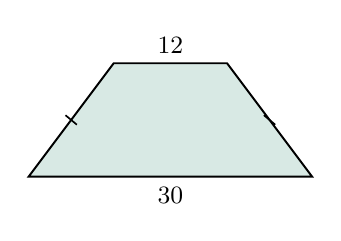
\begin{tikzpicture}[x=0.12cm,y=0.12cm]
\fill[badge!45] (0,0)--(30,0)--(21,12)--(9,12)--cycle;
\draw[line width=0.7pt] (0,0)--(30,0)--(21,12)--(9,12)--cycle;
\node[above,font=\small] at (15,12) {12};
\node[below,font=\small] at (15,0) {30};
\draw[line width=0.6pt] (3.9,6.5)--(5.1,5.5); \draw[line width=0.6pt] (24.9,6.5)--(26.1,5.5);
\end{tikzpicture}}\par\vspace{2.2mm}
\hspace*{7mm}(A)\ $315$\\[1.8mm]
\hspace*{7mm}(B)\ $504$\\[1.8mm]
\hspace*{7mm}(C)\ $189$\\[1.8mm]
\hspace*{7mm}(D)\ $252$
\vfill}}
\end{textblock*}
\clearpage

% ===== Module 2, page 1 =====
\topicheader{9}{Mock Test 9}
\pagefooter{218}
\colrule{34}{236}
\mbox{}%
\pagekicker{Mock 9 \textperiodcentered{} Module 2 \textperiodcentered{} 22 questions \textperiodcentered{} 35 minutes}{Questions 1--8}
\begin{textblock*}{\COLW}(\LCOL,34mm)
{\fontsize{10.4}{13.4}\selectfont
\parbox[t][233mm][t]{\COLW}{%
\noindent\pnum{1} A theater manager packs 5 identical boxes of programs and also adds 12 loose programs, for a total of 112 programs. How many programs are in each box?\par\vspace{2.2mm}
\hspace*{7mm}(A)\ $24.8$\\[1.8mm]
\hspace*{7mm}(B)\ $22.4$\\[1.8mm]
\hspace*{7mm}(C)\ $20$\\[1.8mm]
\hspace*{7mm}(D)\ $100$
\vfill

\noindent\pnum{2} The function $g$ is defined by $g(x)=3\cdot2^{x}$. What is the value of $g(4)-g(2)$?\par\vspace{2.2mm}
\hspace*{7mm}(A)\ $36$\\[1.8mm]
\hspace*{7mm}(B)\ $12$\\[1.8mm]
\hspace*{7mm}(C)\ $24$\\[1.8mm]
\hspace*{7mm}(D)\ $48$
\vfill

\noindent\pnum{3} A shipping container can hold at most 26.5 metric tons of cargo. Each crate weighs 1,250 pounds. If 1 metric ton is 1,000 kilograms and 1 kilogram is 2.2 pounds, what is the greatest number of crates that can be loaded without exceeding the weight limit?\gridbox
\vfill

\noindent\pnum{4} Which of the following is equivalent to $\frac{1}{4}x^{2}-3x+9$?\par\vspace{2.2mm}
\hspace*{7mm}(A)\ $\left(\dfrac{1}{2}x+3\right)^{2}$\\[1.8mm]
\hspace*{7mm}(B)\ $\left(\dfrac{1}{4}x-3\right)^{2}$\\[1.8mm]
\hspace*{7mm}(C)\ $\left(\dfrac{1}{2}x-9\right)^{2}$\\[1.8mm]
\hspace*{7mm}(D)\ $\left(\dfrac{1}{2}x-3\right)^{2}$
\vfill}}
\end{textblock*}
\begin{textblock*}{\COLW}(\RCOL,34mm)
{\fontsize{10.4}{13.4}\selectfont
\parbox[t][233mm][t]{\COLW}{%
\noindent\pnum{5} A rectangular lawn measures 18 meters by 12 meters. A path of uniform width is built around the lawn, so the lawn and the path together form a larger rectangle. The area of the path alone equals the area of the lawn. What is the width of the path, in meters?\par\vspace{2.2mm}
\hspace*{7mm}(A)\ $6$\\[1.8mm]
\hspace*{7mm}(B)\ $3$\\[1.8mm]
\hspace*{7mm}(C)\ $18$\\[1.8mm]
\hspace*{7mm}(D)\ $1.5$
\vfill

\noindent\pnum{6} A map uses a coordinate grid whose units are kilometers. A survey drone flies in a straight line at a constant speed. At 2:00 p.m. it is at $(3,-1)$, and at 2:30 p.m. it is at $(9,3)$. At the moment the drone's $x$-coordinate is 21, what is its $y$-coordinate?\par\vspace{2.2mm}
\hspace*{7mm}(A)\ $11$\\[1.8mm]
\hspace*{7mm}(B)\ $15$\\[1.8mm]
\hspace*{7mm}(C)\ $7$\\[1.8mm]
\hspace*{7mm}(D)\ $14$
\vfill

\noindent\pnum{7} A wildlife biologist tags 80 fish in a lake and releases them. Several days later she catches a random sample of 150 fish from the lake and finds that 12 of them are tagged. Assuming the proportion of tagged fish in the sample equals the proportion of tagged fish in the whole lake, about how many fish are in the lake?\par\vspace{2.2mm}
\hspace*{7mm}(A)\ $960$\\[1.8mm]
\hspace*{7mm}(B)\ $1{,}800$\\[1.8mm]
\hspace*{7mm}(C)\ $1{,}000$\\[1.8mm]
\hspace*{7mm}(D)\ $218$
\vfill

\noindent\pnum{8} A research thermometer uses a new scale $T$ that is a linear function of the Fahrenheit scale. Water freezes at $32^{\circ}$F, which reads $20^{\circ}$T, and boils at $212^{\circ}$F, which reads $220^{\circ}$T. What is the reading, in degrees T, when the temperature is $98.6^{\circ}$F?\gridbox
\vfill}}
\end{textblock*}
\clearpage

% ===== Module 2, page 2 =====
\topicheader{9}{Mock Test 9}
\pagefooter{219}
\colrule{34}{236}
\mbox{}%
\pagekicker{Mock 9 \textperiodcentered{} Module 2 \textperiodcentered{} 22 questions \textperiodcentered{} 35 minutes}{Questions 9--15}
\begin{textblock*}{\COLW}(\LCOL,34mm)
{\fontsize{10.4}{13.4}\selectfont
\parbox[t][233mm][t]{\COLW}{%
\noindent\pnum{9} Plant A is 10 centimeters tall today and grows 4 centimeters each month. Plant B is also 10 centimeters tall today, and its height increases by 20\% each month. At the end of which month is Plant B first taller than Plant A?\par\vspace{2.2mm}
\hspace*{7mm}(A)\ Month 6\\[1.8mm]
\hspace*{7mm}(B)\ Month 8\\[1.8mm]
\hspace*{7mm}(C)\ Month 7\\[1.8mm]
\hspace*{7mm}(D)\ Month 9
\vfill

\noindent\pnum{10} In the figure, two circles share center $O$. A chord of the larger circle is tangent to the smaller circle. The chord has length 24, and the radius of the smaller circle is 5. What is the area of the region between the two circles?\figwrap{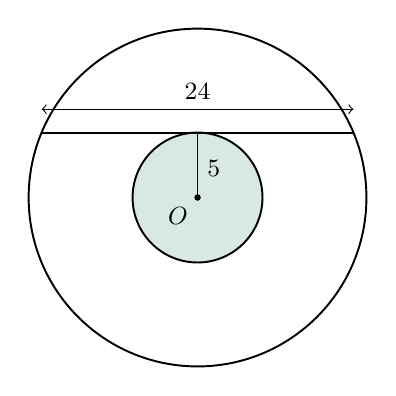
\begin{tikzpicture}[scale=0.165]
\draw[line width=0.7pt] (0,0) circle (13);
\fill[badge!45] (0,0) circle (5);
\draw[line width=0.7pt] (0,0) circle (5);
\draw[line width=0.7pt] (-12,5)--(12,5);
\fill (0,0) circle (0.25); \node[below left,font=\small] at (0,0) {$O$};
\draw[line width=0.5pt] (0,0)--(0,5);
\node[right,font=\small] at (0,2.2) {5};
\draw[line width=0.4pt,<->] (-12,6.8)--(12,6.8);
\node[above,font=\small] at (0,6.8) {24};
\end{tikzpicture}}\par\vspace{2.2mm}
\hspace*{7mm}(A)\ $169\pi$\\[1.8mm]
\hspace*{7mm}(B)\ $576\pi$\\[1.8mm]
\hspace*{7mm}(C)\ $119\pi$\\[1.8mm]
\hspace*{7mm}(D)\ $144\pi$
\vfill

\noindent\pnum{11} A theater sold 200 tickets for a show: adult tickets at \$18, student tickets at \$12, and senior tickets at \$10. The theater sold the same number of student tickets as senior tickets and collected \$3,320 in all. How many adult tickets were sold?\par\vspace{2.2mm}
\hspace*{7mm}(A)\ $160$\\[1.8mm]
\hspace*{7mm}(B)\ $20$\\[1.8mm]
\hspace*{7mm}(C)\ $180$\\[1.8mm]
\hspace*{7mm}(D)\ $40$
\vfill}}
\end{textblock*}
\begin{textblock*}{\COLW}(\RCOL,34mm)
{\fontsize{10.4}{13.4}\selectfont
\parbox[t][233mm][t]{\COLW}{%
\noindent\pnum{12} Three-fourths of a number is 15 more than one-third of the same number. What is one-half of the number?\gridbox
\vfill

\noindent\pnum{13} For the equation $(k^{2}-k-6)x=k^{2}-9$, where $k$ is a constant, for which value of $k$ does the equation have no solution?\par\vspace{2.2mm}
\hspace*{7mm}(A)\ $3$\\[1.8mm]
\hspace*{7mm}(B)\ $-2$\\[1.8mm]
\hspace*{7mm}(C)\ $-3$\\[1.8mm]
\hspace*{7mm}(D)\ $2$
\vfill

\noindent\pnum{14} In the $xy$-plane, the graph of $y=x^{2}+2$ and the graph of $x^{2}+y^{2}=k$, where $k$ is a positive constant, have exactly one point in common. What is the value of $k$?\par\vspace{2.2mm}
\hspace*{7mm}(A)\ $2$\\[1.8mm]
\hspace*{7mm}(B)\ $\dfrac{9}{4}$\\[1.8mm]
\hspace*{7mm}(C)\ $4$\\[1.8mm]
\hspace*{7mm}(D)\ $8$
\vfill

\noindent\pnum{15} In the figure, line $PT$ is tangent at $T$ to a circle with center $O$. Segment $PO$ meets the circle at $A$. If $PT=24$ and $PA=16$, what is the radius of the circle?\figwrap{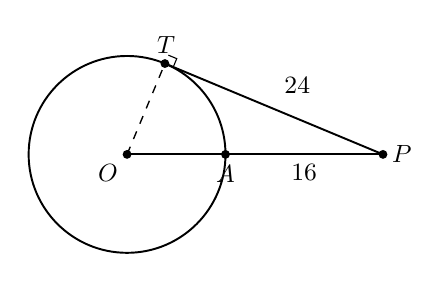
\begin{tikzpicture}[scale=0.125]
\draw[line width=0.7pt] (0,0) circle (10);
\coordinate (O) at (0,0); \coordinate (P) at (26,0); \coordinate (T) at (3.846,9.231); \coordinate (A) at (10,0);
\draw[line width=0.7pt] (P)--(T); \draw[line width=0.7pt] (O)--(P); \draw[line width=0.5pt,dashed] (O)--(T);
\fill (O) circle (0.45); \fill (A) circle (0.45); \fill (T) circle (0.45); \fill (P) circle (0.45);
\node[below left,font=\small] at (O) {$O$}; \node[below,font=\small] at (A) {$A$}; \node[above,font=\small] at (T) {$T$}; \node[right,font=\small] at (P) {$P$};
\node[above right,font=\small] at (15,5.2) {24}; \node[below,font=\small] at (18,0) {16};
\draw[line width=0.4pt] ($(T)+(0.85,-0.35)$)--($(T)+(1.2,0.5)$)--($(T)+(0.35,0.85)$);
\end{tikzpicture}}\gridbox
\vfill}}
\end{textblock*}
\clearpage

% ===== Module 2, page 3 =====
\topicheader{9}{Mock Test 9}
\pagefooter{220}
\colrule{34}{236}
\mbox{}%
\pagekicker{Mock 9 \textperiodcentered{} Module 2 \textperiodcentered{} 22 questions \textperiodcentered{} 35 minutes}{Questions 16--22}
\begin{textblock*}{\COLW}(\LCOL,34mm)
{\fontsize{10.4}{13.4}\selectfont
\parbox[t][233mm][t]{\COLW}{%
\noindent\pnum{16} A set of 7 positive integers has a mean of 10, a median of 9, and a unique mode of 8. What is the greatest possible value of the largest integer in the set?\par\vspace{2.2mm}
\hspace*{7mm}(A)\ $26$\\[1.8mm]
\hspace*{7mm}(B)\ $18$\\[1.8mm]
\hspace*{7mm}(C)\ $40$\\[1.8mm]
\hspace*{7mm}(D)\ $23$
\vfill

\noindent\pnum{17} In the $xy$-plane, the line $y=2x-3$ intersects the parabola $y=x^{2}-5x+k$, where $k$ is a constant, at two points. The $x$-coordinates of these two points differ by 5. What is the value of $k$?\par\vspace{2.2mm}
\hspace*{7mm}(A)\ $3$\\[1.8mm]
\hspace*{7mm}(B)\ $6$\\[1.8mm]
\hspace*{7mm}(C)\ $-3$\\[1.8mm]
\hspace*{7mm}(D)\ $8$
\vfill

\noindent\pnum{18} In a league of 10 teams, every team plays every other team exactly once. A win earns a team 3 points, a draw earns each of the two teams 1 point, and a loss earns 0 points. When all games have been played, the mean number of points per team is 12.5. How many of the games ended in a draw?\par\vspace{2.2mm}
\hspace*{7mm}(A)\ $5$\\[1.8mm]
\hspace*{7mm}(B)\ $20$\\[1.8mm]
\hspace*{7mm}(C)\ $10$\\[1.8mm]
\hspace*{7mm}(D)\ $35$
\vfill}}
\end{textblock*}
\begin{textblock*}{\COLW}(\RCOL,34mm)
{\fontsize{10.4}{13.4}\selectfont
\parbox[t][233mm][t]{\COLW}{%
\noindent\pnum{19} Two delivery drones leave depots at opposite ends of a straight route at the same moment, each flying at its own constant speed toward the other depot. After passing each other, drone A needs 9 more minutes to reach the far depot and drone B needs 4 more minutes. How many minutes after takeoff did the drones pass each other?\gridbox
\vfill

\noindent\pnum{20} The table gives three values of the quadratic function $f$. The function $g$ is defined by $g(x)=f\left(\dfrac{x-3}{2}\right)$. What is the sum of the zeros of $g$?\figwrap{\begin{tabular}{|c|c|c|c|}
\hline
$x$ & 0 & 1 & 3\\\hline
$f(x)$ & 16 & 7 & $-5$\\\hline
\end{tabular}}\par\vspace{2.2mm}
\hspace*{7mm}(A)\ $20$\\[1.8mm]
\hspace*{7mm}(B)\ $26$\\[1.8mm]
\hspace*{7mm}(C)\ $16$\\[1.8mm]
\hspace*{7mm}(D)\ $11$
\vfill

\noindent\pnum{21} In the figure, a chord is 5 units from the center $O$ of a circle with radius 10. What is the area of the shaded region, which lies on the side of the chord away from $O$?\figwrap{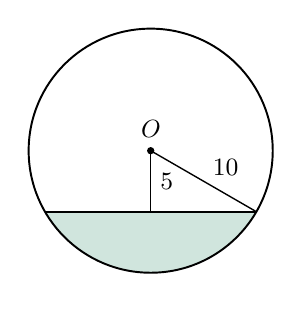
\begin{tikzpicture}[scale=0.155]
\fill[badge!55] (-8.66,-5) arc (210:330:10) -- cycle;
\draw[line width=0.7pt] (0,0) circle (10);
\draw[line width=0.7pt] (-8.66,-5)--(8.66,-5);
\fill (0,0) circle (0.3); \node[above,font=\small] at (0,0.2) {$O$};
\draw[line width=0.5pt] (0,0)--(0,-5); \node[right,font=\small] at (0,-2.5) {5};
\draw[line width=0.5pt] (0,0)--(8.66,-5); \node[above right,font=\small] at (4.3,-2.9) {10};
\end{tikzpicture}}\par\vspace{2.2mm}
\hspace*{7mm}(A)\ $\dfrac{100\pi}{3}-50\sqrt{3}$\\[1.8mm]
\hspace*{7mm}(B)\ $\dfrac{50\pi}{3}-25\sqrt{3}$\\[1.8mm]
\hspace*{7mm}(C)\ $\dfrac{100\pi}{3}+25\sqrt{3}$\\[1.8mm]
\hspace*{7mm}(D)\ $\dfrac{100\pi}{3}-25\sqrt{3}$
\vfill

\noindent\pnum{22} For how many integer values of $k$ does the equation $|x^{2}-4x-5|=k$ have exactly four distinct real solutions?\gridbox
\vfill}}
\end{textblock*}
\clearpage

\end{document}
